\section{Correlation}\label{sec:corr}

Calculating the correlation between the score of each zero-cost proxy and the validation accuracy is a logical approach to understanding the impact of the zero-cost proxies. Spearman Rank Correlation is a non-parametric statistical test that measures the strength and direction of the association between two ranked variables \autocite{hauke2011comparison}. The Spearman Rank does not assume a linear relationship between the two variables. It is suitable for cases where the connection between the validation accuracy and the zero-cost proxy may not be linear. Additionally, the metric is less vulnerable to outliers because it focuses on the rank of the variables rather than their raw values.

Pearson correlation coefficient is the most commonly used correlation coefficient. The coefficient provides insights into the strength and direction of a linear relationship \autocite{turney2022pearson}. 

However, its utility for our project is limited due to several constraints. First, it assumes the variables in the dataset are normally distributed \autocite{turney2022pearson}. The Shapiro-Wilk test is a statistical test used to check whether a sample of numbers has been drawn from a normally distributed population. The starting assumption (or null hypothesis) is that the population is normally distributed \autocite{shaphiro1965analysis}. The null hypothesis is disregarded if the test's calculated p-value is less than the predetermined alpha level, typically 0.05. Discarding the null hypothesis means we have enough evidence to conclude that the data set under investigation does not exhibit a normal distribution. The Shapiro-Wilk test result for each variable (zero-cost proxy) is shown in \cref{tab:p_values}. 

\begin{table}[h]
\caption{P-values for each variable using the Shapiro-Wilk test}
\centering
\begin{tabular}{lr||lr}
\textbf{ZC-proxy} & \textbf{P-value} & \textbf{ZC-proxy} & \textbf{P-value} \\ \hline
\multicolumn{1}{l|}{\cellcolor{verylightgray}EPE-NAS} & \cellcolor{verylightgray}$<1e-6$ & \multicolumn{1}{l|}{\cellcolor{verylightgray}NAS-WOT} & \cellcolor{verylightgray}$0.003$ \\
\multicolumn{1}{l|}{Fisher} & $< 1e-6$ & \multicolumn{1}{l|}{Params} & $< 1e-6$ \\
\multicolumn{1}{l|}{\cellcolor{verylightgray}Flops} & \cellcolor{verylightgray} $< 1e-6$ & \multicolumn{1}{l|}{\cellcolor{verylightgray}Plain} & \cellcolor{verylightgray} $< 1e-6$ \\
\multicolumn{1}{l|}{Grad Norm} & $< 1e-6$ & \multicolumn{1}{l|}{Snip} & $< 1e-6$ \\
\multicolumn{1}{l|}{\cellcolor{verylightgray}GradSign} & \cellcolor{verylightgray}$< 1e-6$ & \multicolumn{1}{l|}{\cellcolor{verylightgray}Synflow} & \cellcolor{verylightgray}$< 1e-6$ \\
\multicolumn{1}{l|}{Grasp} & $< 1e-6$ & \multicolumn{1}{l|}{Val. acc} & $< 1e-6$ \\
\multicolumn{1}{l|}{\cellcolor{verylightgray}Jacov} & \cellcolor{verylightgray}$< 1e-6$ & \multicolumn{1}{l|}{\cellcolor{verylightgray}Zen} & \cellcolor{verylightgray}$< 1e-6$ \\
\multicolumn{1}{l|}{L2 norm} & $< 1e-6$ & & \\
\end{tabular}
\label{tab:p_values}
\end{table}



The p-values for all variables are smaller than the significance level ($\alpha = 0.05$), as seen in the \cref{tab:p_values}. Therefore, we can disprove the Shapiro-Wilk test's null hypothesis for each variable, showing that the distributions of those variables considerably differ from the normal distribution.

Further, Pearson's correlation is highly sensitive to outliers. A few extreme observations can greatly distort the correlation coefficient, potentially leading to incorrect interpretations. This sensitivity is unwanted given that the zero-cost proxies may contain such outliers, as illustrated in \cref{fig:zero_cost_proxies_outliers}, in which one can observe that the data contains outliers (i.e. Synflow in the bottom left corner). 
\clearpage
\begin{figure}[hp!]
  \centering
  \makebox[\linewidth][c]{%
  \begin{subfigure}{0.4\textwidth}
    \includesvg[width=\textwidth]{figures/zc-proxies/epe_nas.svg}
    \caption{EPE-NAS}
    \label{fig:epe_nas}
  \end{subfigure}
  \begin{subfigure}{0.4\textwidth}
    \includesvg[width=\textwidth]{figures/zc-proxies/fisher.svg}
    \caption{Fisher}
    \label{fig:fisher}
  \end{subfigure}
  \begin{subfigure}{0.4\textwidth}
    \includesvg[width=\textwidth]{figures/zc-proxies/flops.svg}
    \caption{Flops}
    \label{fig:flops}
  \end{subfigure}
  }\\
    \makebox[\linewidth][c]{%
  \begin{subfigure}{0.4\textwidth}
    \includesvg[width=\textwidth]{figures/zc-proxies/grad_norm.svg}
    \caption{Grad Norm}
    \label{fig:grad_norm}
  \end{subfigure}
  \begin{subfigure}{0.4\textwidth}
    \includesvg[width=\textwidth]{figures/zc-proxies/grad_sign.svg}
    \caption{GradSign}
    \label{fig:grad_sign}
  \end{subfigure}
  \begin{subfigure}{0.4\textwidth}
    \includesvg[width=\textwidth]{figures/zc-proxies/grasp.svg}
    \caption{Grasp}
    \label{fig:grasp}
  \end{subfigure}
    }\\
        \makebox[\linewidth][c]{%
  \begin{subfigure}{0.4\textwidth}
    \includesvg[width=\textwidth]{figures/zc-proxies/jacov.svg}
    \caption{Jacov}
    \label{fig:jacov}
  \end{subfigure}
  \begin{subfigure}{0.4\textwidth}
    \includesvg[width=\textwidth]{figures/zc-proxies/l2_norm.svg}
    \caption{L2 Norm}
    \label{fig:l2_norm}
  \end{subfigure}
  \begin{subfigure}{0.4\textwidth}
    \includesvg[width=\textwidth]{figures/zc-proxies/nwot.svg}
    \caption{NAS-WOT}
    \label{fig:nwot}
  \end{subfigure}
    }\\
      \makebox[\linewidth][c]{%
  \begin{subfigure}{0.4\textwidth}
    \includesvg[width=\textwidth]{figures/zc-proxies/params.svg}
    \caption{Params}
    \label{fig:params}
  \end{subfigure}
  \begin{subfigure}{0.4\textwidth}
    \includesvg[width=\textwidth]{figures/zc-proxies/plain.svg}
    \caption{Plain}
    \label{fig:plain}
  \end{subfigure}
  \begin{subfigure}{0.4\textwidth}
    \includesvg[width=\textwidth]{figures/zc-proxies/snip.svg}
    \caption{SNIP}
    \label{fig:snip}
  \end{subfigure}
    }\\
      \makebox[\linewidth][c]{%
  \begin{subfigure}{0.4\textwidth}
    \includesvg[width=\textwidth]{figures/zc-proxies/synflow.svg}
    \caption{Synflow}
    \label{fig:synflow}
  \end{subfigure}
  \begin{subfigure}{0.4\textwidth}
    \includesvg[width=\textwidth]{figures/zc-proxies/zen.svg}
    \caption{Zen}
    \label{fig:zen}
  \end{subfigure}
      }\\
  \caption{Each zero-cost proxy normalised with the validation accuracy}
  \label{fig:zero_cost_proxies_outliers}
\end{figure}
\clearpage
% \begin{figure}[h!]
%   \centering
%     \begin{adjustbox}{width=1.2\columnwidth,center}
%   \begin{tabular}{ccc}
%     \includesvg[width=0.5\textwidth]{figures/zc-proxies/epe_nas.svg} &
%     \includesvg[width=0.5\textwidth]{figures/zc-proxies/fisher.svg} &
%     \includesvg[width=0.5\textwidth]{figures/zc-proxies/flops.svg} \\
%     \includesvg[width=0.5\textwidth]{figures/zc-proxies/grad_norm.svg} &
%     \includesvg[width=0.5\textwidth]{figures/zc-proxies/grad_sign.svg} &
%     \includesvg[width=0.5\textwidth]{figures/zc-proxies/grasp.svg} \\
%     \includesvg[width=0.5\textwidth]{figures/zc-proxies/jacov.svg} &
%     \includesvg[width=0.5\textwidth]{figures/zc-proxies/l2_norm.svg} &
%     \includesvg[width=0.5\textwidth]{figures/zc-proxies/nwot.svg} \\
%     \includesvg[width=0.5\textwidth]{figures/zc-proxies/params.svg} &
%     \includesvg[width=0.5\textwidth]{figures/zc-proxies/plain.svg} &
%     \includesvg[width=0.5\textwidth]{figures/zc-proxies/snip.svg} \\
%     \includesvg[width=0.5\textwidth]{figures/zc-proxies/synflow.svg} &
%     \includesvg[width=0.5\textwidth]{figures/zc-proxies/zen.svg} 
%   \end{tabular}
%   \end{adjustbox}
%   \caption{Each zero-cost proxy normalised with the validation accuracy}
%   \label{fig:zero_cost_proxies_outliers}
% \end{figure}

These findings are all pointing in favour of using the Spearman Rank. Lastly, the Pearson correlation coefficient relies on the actual values of the variables, whereas our focus is more on their rankings, which makes the Spearman rank correlation a more suitable measure for our project.




The Spearman Rank Correlation is denoted by the symbol $\rho$ (rho) and ranges from -1 to 1, where -1 indicates a perfect negative relationship, 1 indicates a perfect positive relationship, and 0 shows no connection, as illustrated in \cref{fig:correlations_illustrated} \autocite{laerdstatistics}.  

\begin{figure}[h]
\centering
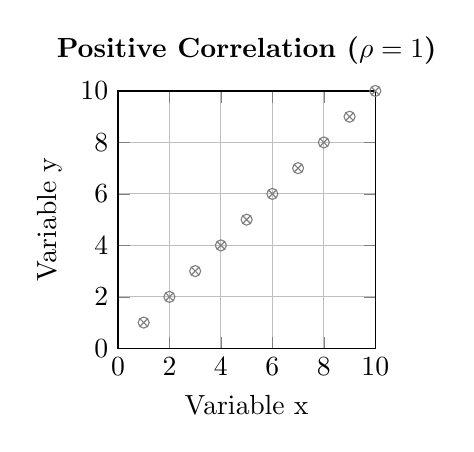
\begin{tikzpicture}
\begin{axis}[
    title={\textbf{Positive Correlation ($\rho = 1$)}},
    xlabel={Variable x},
    ylabel={Variable y},
    xmin=0, xmax=10,
    ymin=0, ymax=10,
    xtick={0,2,4,6,8,10},
    ytick={0,2,4,6,8,10},
    grid=major,
    legend pos=south east,
    width=0.4\textwidth,
    height=0.4\textwidth,
]
\addplot[
    only marks,
    mark=otimes,
    color=gray,
] coordinates {
(1,1)(2,2)(3,3)(4,4)(5,5)(6,6)(7,7)(8,8)(9,9)(10,10)
};
\end{axis}
\end{tikzpicture}
\hspace{1cm}
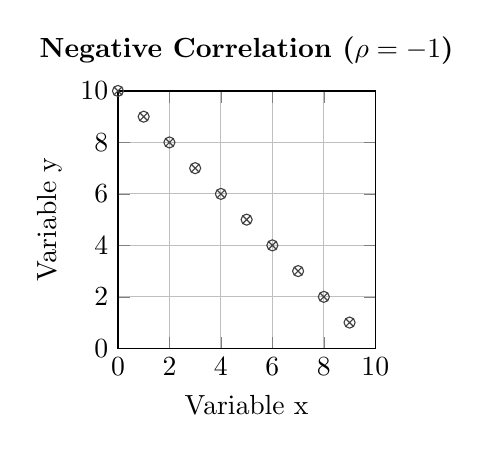
\begin{tikzpicture}
\begin{axis}[
    title={\textbf{Negative Correlation ($\rho = -1$)}},
    xlabel={Variable x},
    ylabel={Variable y},
    xmin=0, xmax=10,
    ymin=0, ymax=10,
    xtick={0,2,4,6,8,10},
    ytick={0,2,4,6,8,10},
    grid=major,
    legend pos=south east,
    width=0.4\textwidth,
    height=0.4\textwidth,
]
\addplot[
    only marks,
    mark=otimes,
    color=darkgray,
] coordinates {
(9,1)(8,2)(7,3)(6,4)(5,5)(4,6)(3,7)(2,8)(1,9)(0,10)
};
\end{axis}
\end{tikzpicture}
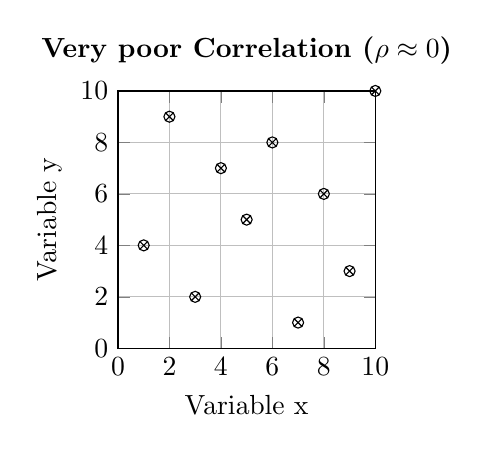
\begin{tikzpicture}
\begin{axis}[
    title={\textbf{Very poor Correlation ($\rho \approx 0$)}},
    xlabel={Variable x},
    ylabel={Variable y},
    xmin=0, xmax=10,
    ymin=0, ymax=10,
    xtick={0,2,4,6,8,10},
    ytick={0,2,4,6,8,10},
    grid=major,
    legend pos=south east,
    width=0.4\textwidth,
    height=0.4\textwidth,
]
\addplot[
    only marks,
    mark=otimes,
    color=black,
] coordinates {
(1,4)(2,9)(3,2)(4,7)(5,5)(6,8)(7,1)(8,6)(9,3)(10,10)
};
\end{axis}
\end{tikzpicture}

\caption{Scatter plots illustrating perfect positive, perfect negative correlations and very poor correlation}
\label{fig:correlations_illustrated}
\end{figure}

Spearman Rank Correlation works by calculating the difference in ranks of the two variables for each observation, then squaring these differences and summing them up, as given in \cref{eq:spearman}. 

\begin{equation} 
    \rho = 1 - \frac{6 \sum d_i^2}{n(n^2 - 1)}, 
    \label{eq:spearman}
 \end{equation}

where $d_i$ is the difference in ranks for each observation, and $n$ is the number of observations.

According to \cite{spear}, Spearman's correlation can generally be described using guidelines from \cref{tab:correlation}. 

\begin{table}[ht]
\caption{Guidelines for interpreting Spearman's correlation}
\centering
\begin{tabular}{lc}
\textbf{Correlation coefficient} & \textbf{Strength of correlation} \\ \hline
\multicolumn{1}{l|}{.00-.19} & Very weak \\
\multicolumn{1}{l|}{\cellcolor{verylightgray}.20-.39} & \cellcolor{verylightgray}Weak \\
\multicolumn{1}{l|}{.40-.59} & Moderate \\
\multicolumn{1}{l|}{\cellcolor{verylightgray}.60-.79} & \cellcolor{verylightgray}Strong \\
\multicolumn{1}{l|}{.80-1.0} & Very strong \\
\end{tabular}

\label{tab:correlation}
\end{table}


In the context of zero-cost proxies and validation accuracy, Spearman Rank Correlation can be used to determine whether there is a monotonic relationship between the two. A positive correlation would indicate that as the zero-cost proxy improves, so does the validation accuracy, while a negative correlation would imply an inverse relationship. A correlation near zero would suggest that the two variables have little or no association. 



